\documentclass[11pt,a4paper]{article}
\usepackage{fontspec}
\setmainfont{TeX Gyre Pagella}
\newfontfamily\headfont{Inter}[UprightFont=*-ExtraBold,BoldFont=*-ExtraBold,Extension=.otf,Path=/usr/share/fonts/opentype/inter/]
\usepackage[a4paper,margin=2.3cm]{geometry}
\usepackage{graphicx,booktabs,float,caption,array,xcolor,longtable}
\usepackage[hidelinks]{hyperref}
\usepackage{titlesec}
\usepackage[round]{natbib}
\usepackage{setspace}
\setstretch{1.05}
\renewcommand{\topfraction}{0.9}
\renewcommand{\bottomfraction}{0.8}
\renewcommand{\textfraction}{0.1}
\renewcommand{\floatpagefraction}{0.75}
\setlength{\parindent}{0pt}
\setlength{\parskip}{0.55em}
\titleformat{\section}{\headfont\Large}{\thesection}{0.8em}{}
\titleformat{\subsection}{\headfont\large}{\thesubsection}{0.8em}{}
\captionsetup{font=small,labelfont=bf}
\urlstyle{same}
\hypersetup{pdftitle={Styles in Stone: The World's Architectural Styles in Wikidata, Mapped Through Time},pdfauthor={Tristan Hotham}}

\begin{document}
\begin{center}
{\Large\bfseries Styles in Stone\par}
\vspace{0.4em}
{\large The world's architectural styles in Wikidata, mapped through time\par}
\vspace{1.2em}
{\large Tristan Hotham\par}
\vspace{0.3em}
{\small Independent researcher\\
ORCID: 0000-0003-4931-9349\\
DOI: \href{https://doi.org/10.5281/zenodo.23842989}{https://doi.org/10.5281/zenodo.23842989}\par}
\vspace{0.8em}
2026
\end{center}

\begin{quote}
\small
\begin{center}\textbf{Abstract}\end{center}
Architectural styles belong to times and places, and then travel. I map the architectural styles recorded in Wikidata for 180,451 buildings and structures with coordinates, which carry 1,314 different style labels. I group the labels into 25 families with a mapping table checked by hand for every style used by 20 or more buildings (covering 99\% of style statements), flag revival styles, and place the 86,148 dated buildings (48\%) in centuries. The textbook sequence emerges from the data unprompted: Romanesque is 63\% of dated buildings from the 1100s, Gothic 72\% of the 1300s, Renaissance 43\% of the 1500s, Baroque and Rococo 51\% of the 1700s, and revival styles make up 42\% of the 1800s. Gothic Revival, with 10,776 buildings in 97 countries, can be followed from Britain (first tenth of precisely dated buildings begun by 1832) to Canada, Australia, the United States and New Zealand. Neoclassical, the largest family, is the most common family in 6 of 53 national capitals with enough buildings to compare. The record is very uneven: the United States and Spain hold 43\% of the buildings, Europe 68\% and Africa 0.4\%, and about a fifth of dates are century-precision values. The atlas maps what Wikidata knows, and is explicit about what it does not.

\textbf{Keywords:} architecture; architectural styles; Gothic Revival; Neoclassical; Wikidata; open data; historical geography; mapping
\end{quote}

\section{Introduction}
Every European town can be read as a sequence of styles: round-arched Romanesque churches, Gothic cathedrals, Renaissance and Baroque palaces, Neoclassical public buildings, the eclectic and revival streets of the nineteenth century, Art Nouveau and Art Deco, and the modernist and Brutalist buildings of the twentieth. Styles also travelled. Gothic returned as Gothic Revival across Britain's settler colonies and the Americas, Greek temple fronts became the courthouses and banks of the United States, and the International Style spread worldwide.

Architectural history describes these movements through canonical buildings. Open data offer a different and much broader, if shallower, view. Wikidata \citep{wikidata}, the collaborative knowledge base behind Wikipedia, records an `architectural style' (property P149) for well over a hundred thousand buildings and structures, many of them ordinary churches, houses and farm buildings loaded from national heritage registers. This study asks what that record shows when the styles are grouped into families, placed on a map and sorted by date, and how far the shape of the record reflects who has entered it.

The result is an interactive atlas (\url{https://maps.tristanhotham.com/architecture-styles/}) with a time slider, a `dominant style' view and search. This paper describes the data, the family mapping and the date handling, reports the main patterns, and sets out the limits of the source.

\section{Data}
All Wikidata extracts were retrieved through the QLever SPARQL engine \citep{qlever} in 2026.

\textbf{Buildings.} Every item with at least one architectural style (P149) and coordinates (P625): 180,451 items carrying 196,135 style statements. For each I kept the coordinates (the first point where an item has several), the English label (85\% have one), the number of sitelinks (wiki pages about the item in any language), the country (P17), the earliest inception date (P571) and the classes it is an instance of (P31). The most common classes are church building (37,898 as first class) and house (24,796); a few items are monuments, bridges, districts or whole towns.

\textbf{Styles.} For each of the 1,314 styles in use, its English label, its parents (P279, subclass of) and wholes (P361, part of), and its start and end dates where given.

\textbf{Geography.} Natural Earth 1:50m countries and populated places \citep{naturalearth}. A building's country is its Wikidata country where that has an ISO code, otherwise the country under its point.

\begin{table}[tbp]\centering\small\caption{Sources, what was kept and licences.}\label{tab:sources}\begin{tabular}{>{\raggedright\arraybackslash}p{3.0cm}>{\raggedright\arraybackslash}p{7.2cm}r>{\raggedright\arraybackslash}p{2.2cm}}\toprule Source & Kept & Records & Licence\\\midrule
Wikidata & Items with an architectural style (P149) and coordinates & 180,451 & CC0\\
Wikidata & Style statements on those items & 196,135 & CC0\\
Wikidata & Styles in use, with parents and part-of links & 1,314 & CC0\\
Wikidata & Items with an inception date & 86,148 & CC0\\
Natural Earth & Countries (1:50m) and populated places & 240 / 2,517 & Public domain\\
\bottomrule\end{tabular}\end{table}

\section{Methods}
\subsection{Style families}
The 1,314 labels range from broad movements (`baroque architecture', 13,536 buildings) to narrow regional and technical terms (`Kasuga-zukuri', `Brabantine Gothic', `gable roof'). I grouped them into 25 families and an `Other or general' group (Table~\ref{tab:fam}). Each style was assigned in three steps. First, every style used by 20 or more buildings was decided by hand (478 styles, 99\% of all style statements), reading its label, parents and a sample of its buildings. Second, smaller styles were assigned by words in their English labels (417 styles). Third, the remainder took the family of the nearest classified ancestor in the P279 and P361 hierarchy (61 styles). The 358 styles left over, all rare, join `Other or general', as do general or technical labels such as `medieval architecture', `industrial architecture', roof forms and classical orders. The complete table, with the method used for each style, is published with the data.

A style is a \emph{revival} when it re-uses an earlier style's forms in a later period. Revival styles keep the family of the style they revive and carry a flag: Gothic Revival is Gothic, Greek Revival Neoclassical, Moorish Revival Islamic, and Colonial, Spanish Colonial and Mission Revival Colonial. Some families combine movements that historians keep apart: socialist realist and Stalinist classicism are counted as Neoclassical revivals, and Noucentisme, the Catalan classicism of the early twentieth century, as historicist.

A building with several styles (9,731 have styles in more than one family) is coloured by its most specific style, the one used by the fewest buildings, ignoring `Other or general' where possible.

\subsection{Dates}
Inception (P571) is the date a building was begun or an institution founded. The extract gives the date but not its precision, and the distribution of years shows that this matters: 2,374 buildings are dated exactly 2000 against 51 for 1999 and 56 for 2001, and 1,229 exactly 1500 against 142 for 1501. Wikidata stores a century-precision date as the last year of the century (`20th century' is 2000), so I read every year ending in 00 (21\% of dated buildings) as the middle of the century it ends. A sensitivity check reading them as written is reported below.

Inception can also predate the present building: a medieval parish whose church was rebuilt in the nineteenth century keeps its founding date. I therefore set a plausible earliest year for each family and revival (for example 1740 for Gothic Revival, 1880 for Art Nouveau, 1945 for Brutalist) and leave buildings dated more than 25 years earlier out of the time analysis (3,166 buildings, 3.7\% of those dated). 36 dates after 2026 are treated as missing. 82,982 buildings remain in the time analysis.

\subsection{Revivals, capitals and dominance}
For Gothic Revival I take buildings dated to a year (not a round century) from 1740 on, and for each country with at least 15 such buildings report the year by which the first tenth had been begun (the 10th percentile) and the median year. For capitals I count buildings within 15 km of each Natural Earth national capital, keeping capitals with at least 40. The `dominant style' of an area is the family with most buildings, ignoring `Other or general'.

\section{Results}
\subsection{Families}
Neoclassical is the largest family (26,140 buildings), followed by Gothic (22,106), Vernacular (19,150), Historicist and eclectic (18,678) and Baroque and Rococo (17,035) (Figure~\ref{fig:fam}). 36,445 buildings (20\%) are in a revival style; 48.7\% of Gothic buildings are Gothic Revival and 50.4\% of Renaissance buildings are Renaissance Revival or Italianate. The families from outside the European tradition (Islamic, Persian, Ottoman, Mughal and Indo-Islamic, Hindu temple, Chinese and Korean, Japanese, Southeast Asian and Pre-Columbian) hold 5\% of the buildings together.

\begin{figure}[tbp]\centering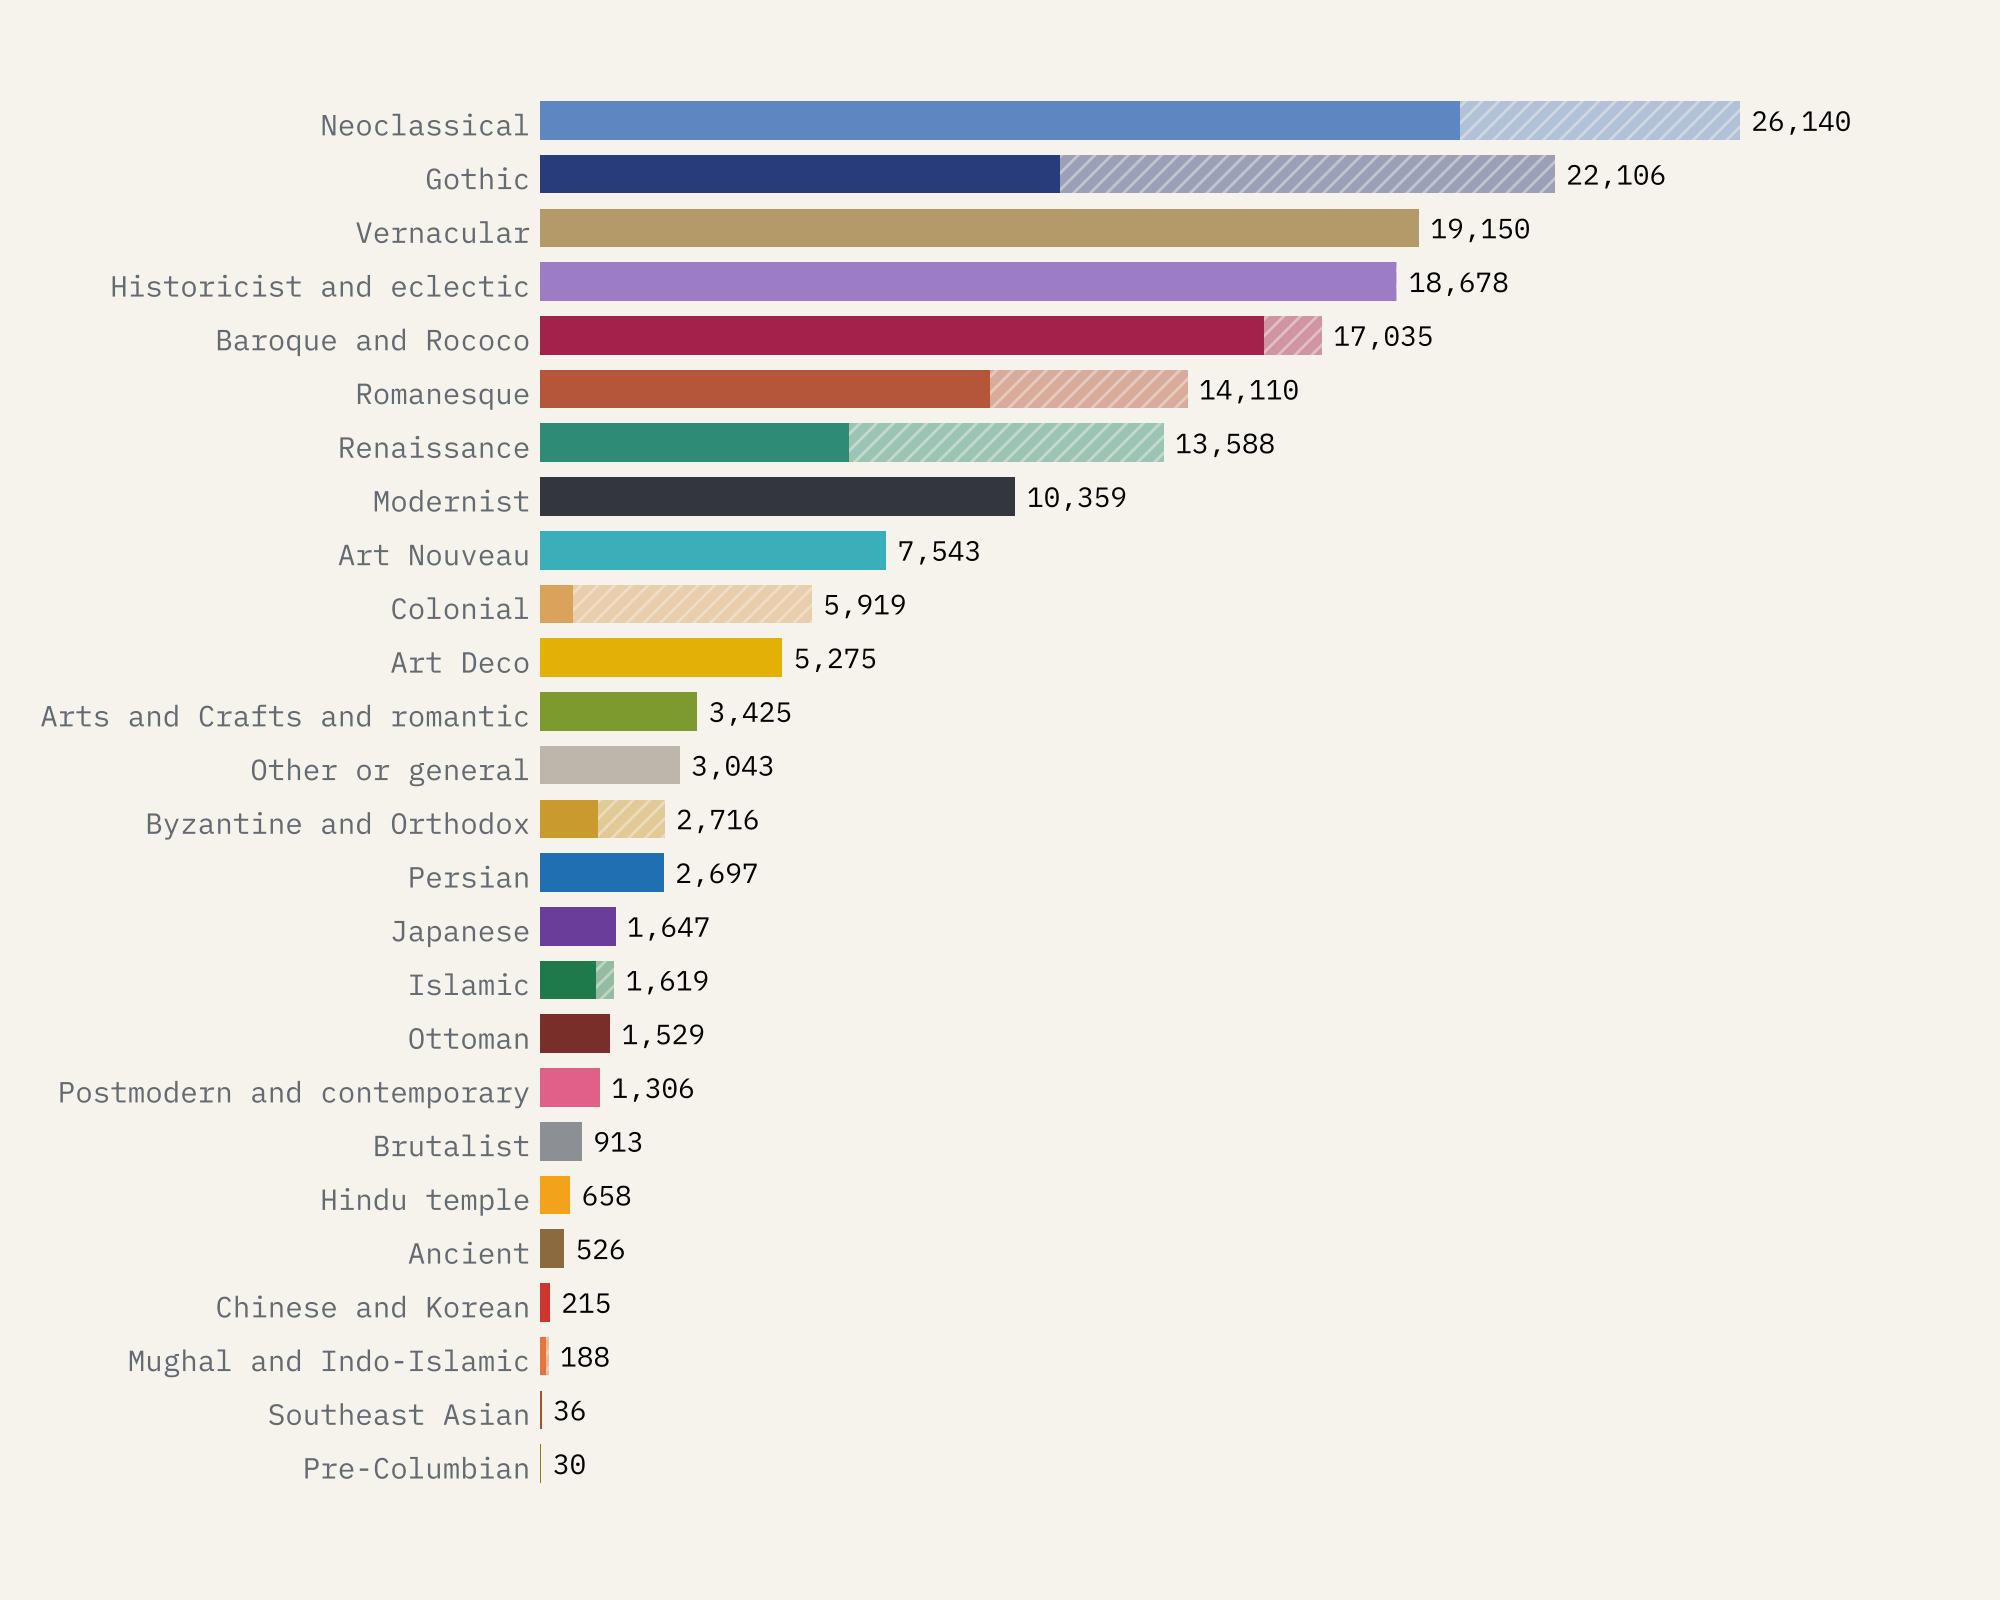
\includegraphics[width=.84\textwidth]{f_families.png}
\caption{Buildings by style family. Hatched: revival styles.}\label{fig:fam}\end{figure}

\begin{table}[tbp]\centering\footnotesize\caption{The style families: buildings, revival buildings, number of Wikidata styles and median year of dated buildings (round-century years read as mid-century; dates earlier than the style left out).}\label{tab:fam}\setlength{\tabcolsep}{4pt}\begin{tabular}{>{\raggedright\arraybackslash}p{3.2cm}>{\raggedright\arraybackslash}p{6.4cm}rrrr}\toprule Family & Includes & Buildings & Revival & Styles & Median\\\midrule
Ancient & Egyptian, Greek, Roman, Persian and other ancient building & 526 & 0 & 32 & 50\\
Byzantine and Orthodox & Byzantine, Armenian, Georgian and Old Russian, with their revivals & 2,716 & 1,453 & 30 & 1875\\
Romanesque & Pre-Romanesque, Romanesque and Norman, with Romanesque Revival & 14,110 & 4,302 & 51 & 1377\\
Gothic & Gothic in all its regional forms, with Gothic Revival & 22,106 & 10,776 & 67 & 1850\\
Renaissance & Renaissance and Mannerist, with Renaissance Revival and Italianate & 13,588 & 6,852 & 57 & 1850\\
Baroque and Rococo & Baroque and Rococo, with baroque revival & 17,035 & 1,258 & 72 & 1750\\
Neoclassical & Classicism, Palladian, Georgian, Federal, Empire and Greek Revival & 26,140 & 6,094 & 62 & 1850\\
Historicist and eclectic & Eclectic, Victorian, Beaux-Arts, Second Empire and Queen Anne & 18,678 & 39 & 71 & 1896\\
Colonial & Colonial building in the Americas and elsewhere, with Colonial and Spanish Colonial Revival & 5,919 & 5,196 & 28 & 1914\\
Arts and Crafts and romantic & Arts and Crafts, Craftsman, Prairie School, rustic and National Romantic & 3,425 & 0 & 27 & 1917\\
Art Nouveau & Art Nouveau, Jugendstil, Secession and Catalan modernisme & 7,543 & 0 & 23 & 1910\\
Art Deco & Art Deco, Moderne and Streamline Moderne & 5,275 & 0 & 11 & 1932\\
Modernist & Modern, functionalist, rationalist, International Style, constructivist and Bauhaus & 10,359 & 0 & 84 & 1948\\
Brutalist & Brutalist architecture & 913 & 0 & 2 & 1970\\
Postmodern and contemporary & Postmodern, high-tech, deconstructivist and contemporary & 1,306 & 0 & 17 & 1999\\
Islamic & Arab, Andalusian, Maghrebi, Mamluk and Mudéjar, with Moorish Revival & 1,619 & 407 & 44 & 1830\\
Persian & Iranian architecture by dynasty: Seljuk, Ilkhanid, Timurid, Safavid, Qajar, Pahlavi & 2,697 & 0 & 19 & 1928\\
Ottoman & Ottoman architecture & 1,529 & 0 & 3 & 1618\\
Mughal and Indo-Islamic & Indo-Islamic and Mughal, with Indo-Saracenic & 188 & 49 & 8 & 1683\\
Hindu temple & Dravidian, Nagara, Kalinga and Bengal temple styles & 658 & 0 & 24 & 1776\\
Chinese and Korean & Chinese and Korean architecture & 215 & 0 & 10 & 1867\\
Japanese & Shinto shrine styles, Buddhist temple styles, kofun and minka & 1,647 & 0 & 56 & 810\\
Southeast Asian & Khmer, Thai, Javanese, Balinese and Malay & 36 & 0 & 13 & 1879\\
Pre-Columbian & Maya, Inca and other Pre-Columbian building, with Mayan Revival & 30 & 19 & 6 & 1927\\
Vernacular & Vernacular, folk, wooden and timber-framed building & 19,150 & 0 & 77 & 1801\\
Other or general & General or technical labels: medieval, industrial, roof shapes, orders & 3,043 & 0 & 420 & 1955\\
\bottomrule\end{tabular}\end{table}

\begin{figure}[tbp]\centering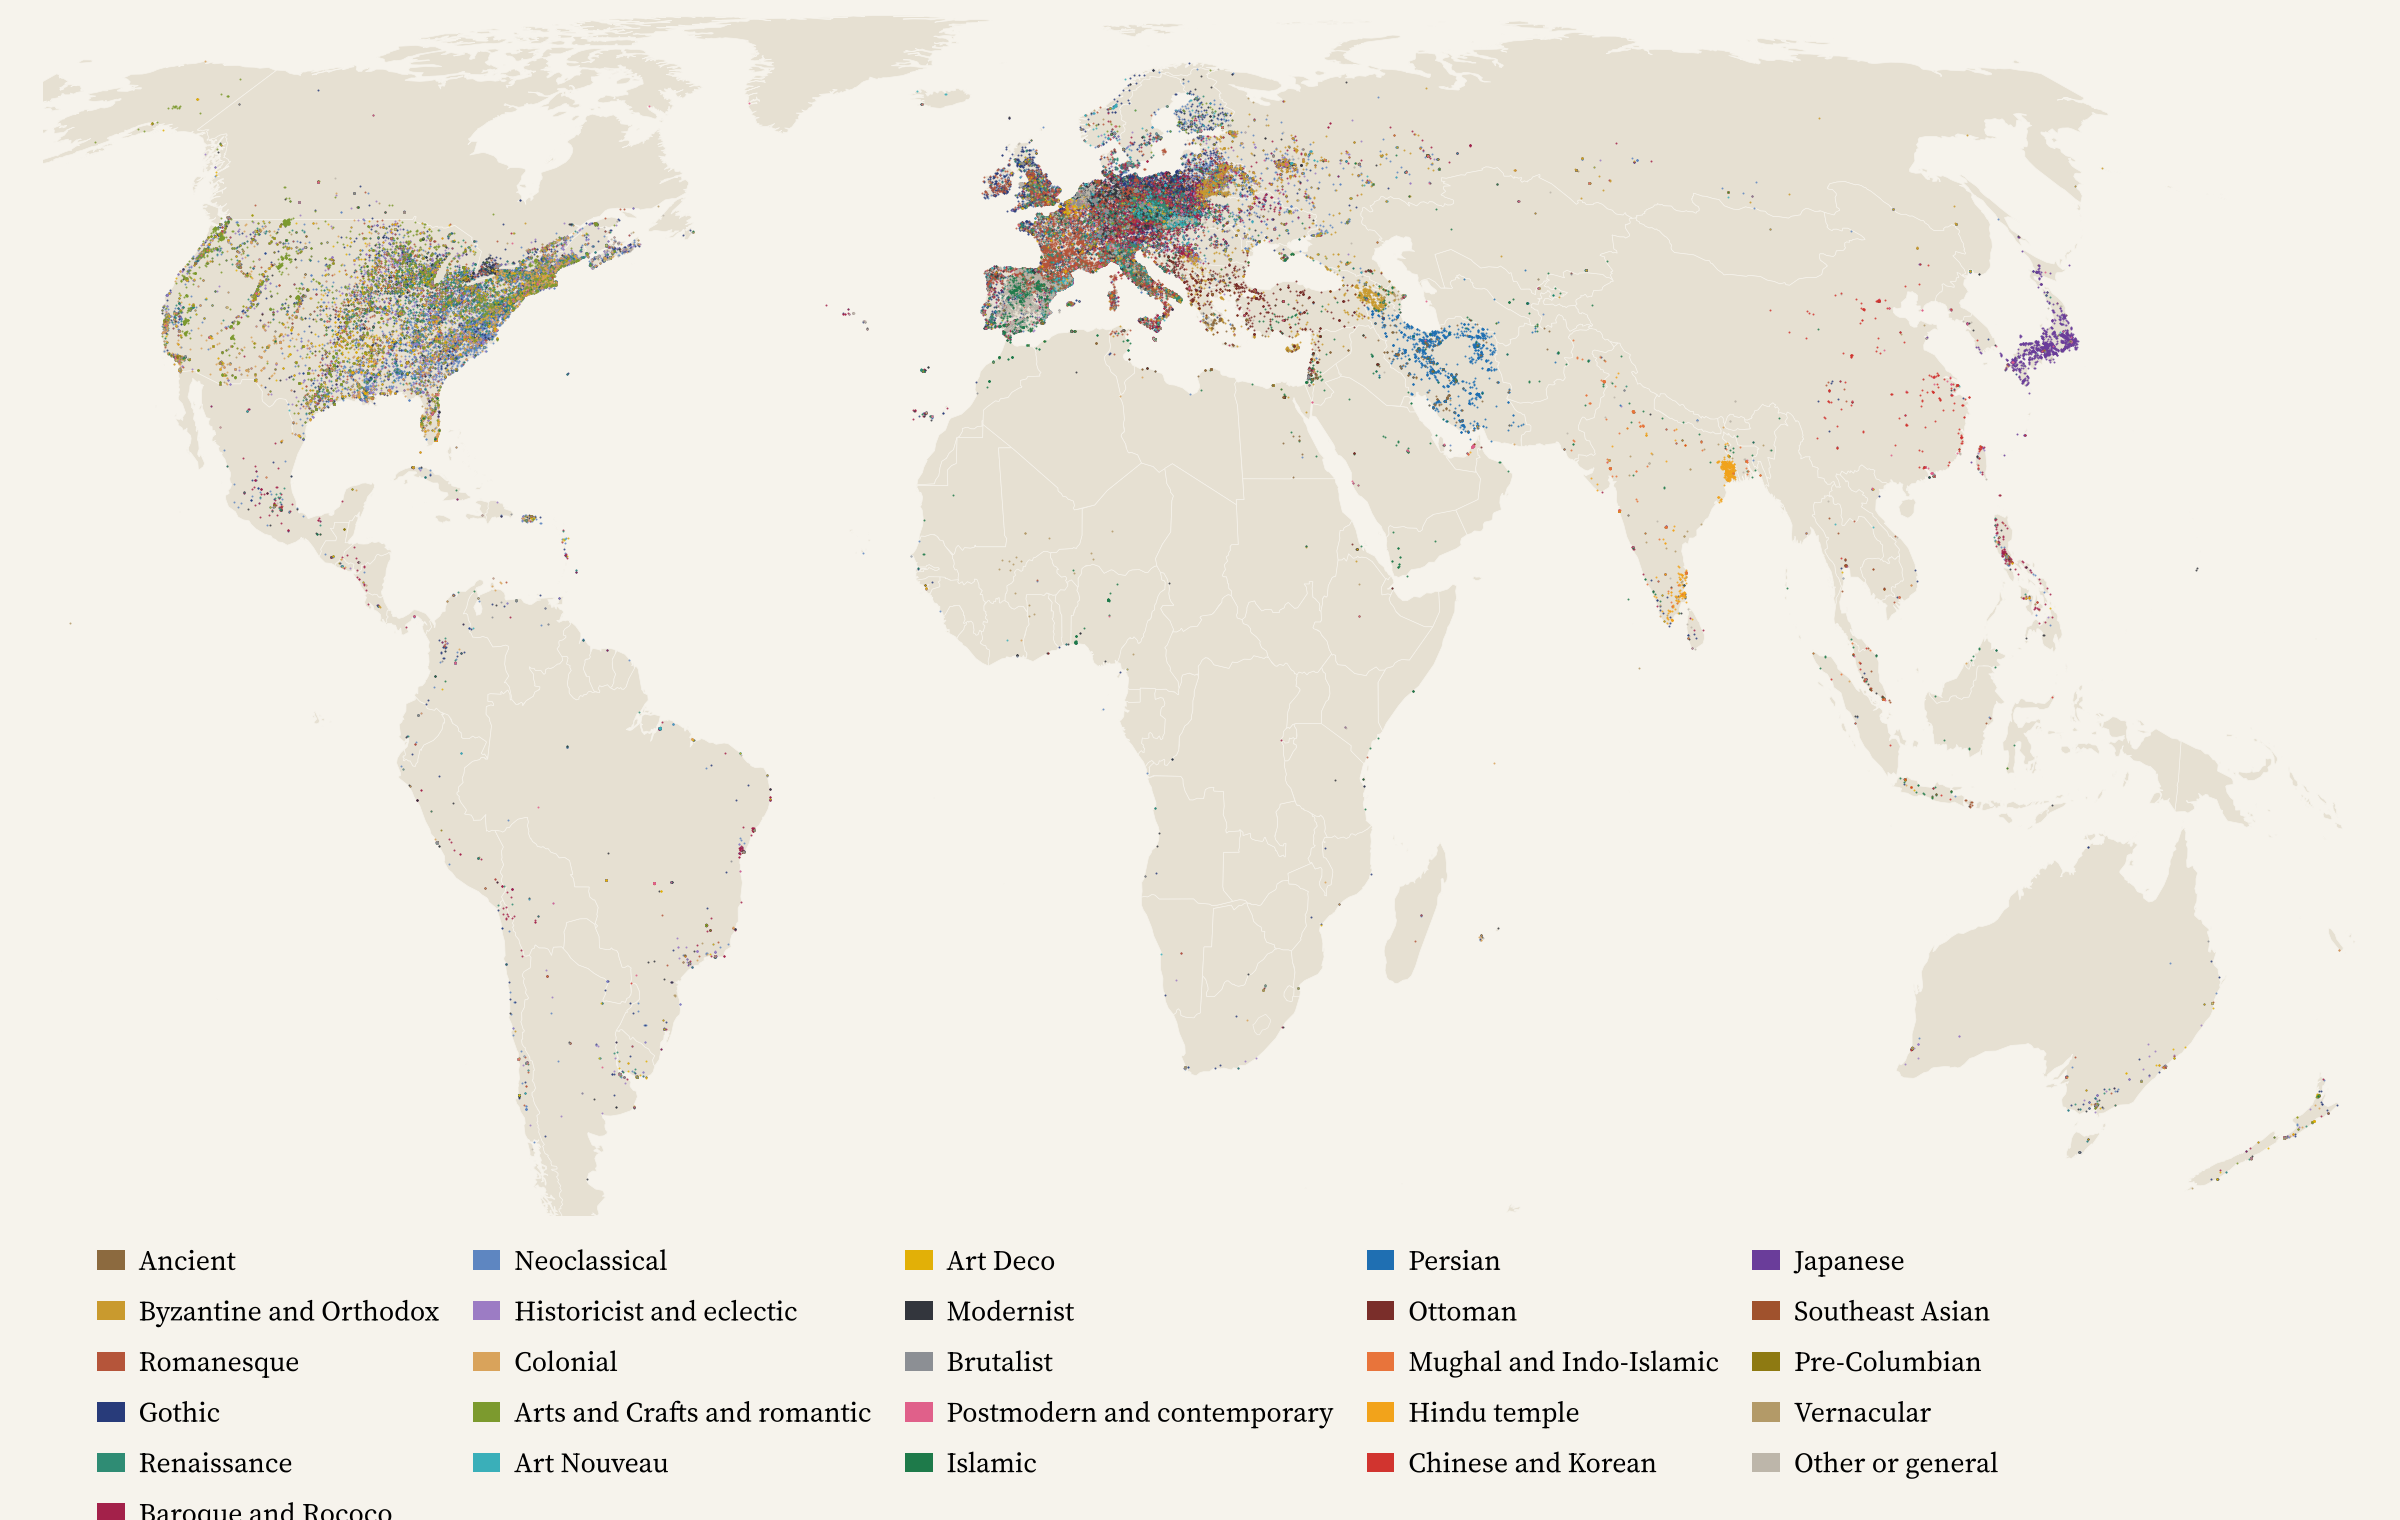
\includegraphics[width=\textwidth]{f_world_map.png}
\caption{All 180,451 buildings, coloured by style family.}\label{fig:world}\end{figure}

\subsection{Through time}
Sorted into centuries, the dated buildings reproduce the conventional sequence of European architecture (Figure~\ref{fig:cent}). Romanesque leads every century from the 800s to the 1100s (63\% in the 1100s); Gothic leads from the 1200s to the 1400s (72\% in the 1300s); Renaissance leads the 1500s (43\%); Baroque and Rococo lead the 1600s and 1700s (51\% in the 1700s); and Neoclassical leads the 1800s (27\%), a century in which revival styles of every kind make up 42\% of dated buildings. The 1900s are the most varied century: Modernist leads with only 17\%, ahead of historicist, Art Deco (12\%) and Art Nouveau (11\%). Since 2000 postmodern and contemporary styles lead (31\%). Before the 1100s every century rests on fewer than a thousand buildings, and Japanese shrine and tomb styles lead from the 300s to the 700s.

The sequence is also geographical (Figure~\ref{fig:eur}). In the 1100s Romanesque covers western and central Europe; by the 1300s Gothic dominates from England to the Baltic; in the 1500s Renaissance leads in Spain, Bohemia and Poland while the Ottoman Balkans differ; the 1700s are Baroque across central Europe, with Neoclassical already ahead in Britain and Scandinavia; the 1800s mix Gothic Revival in Britain with Neoclassical and historicist styles further east; and the 1900s break into Modernist, Art Deco (most visibly in Belgium) and Art Nouveau.

Reading round-century years as written rather than as century-precision dates moves the share of a family in a century by up to 20.2 percentage points and changes the leading family in 3 centuries with at least 50 buildings; the sequence above is unchanged in outline.

\begin{figure}[tbp]\centering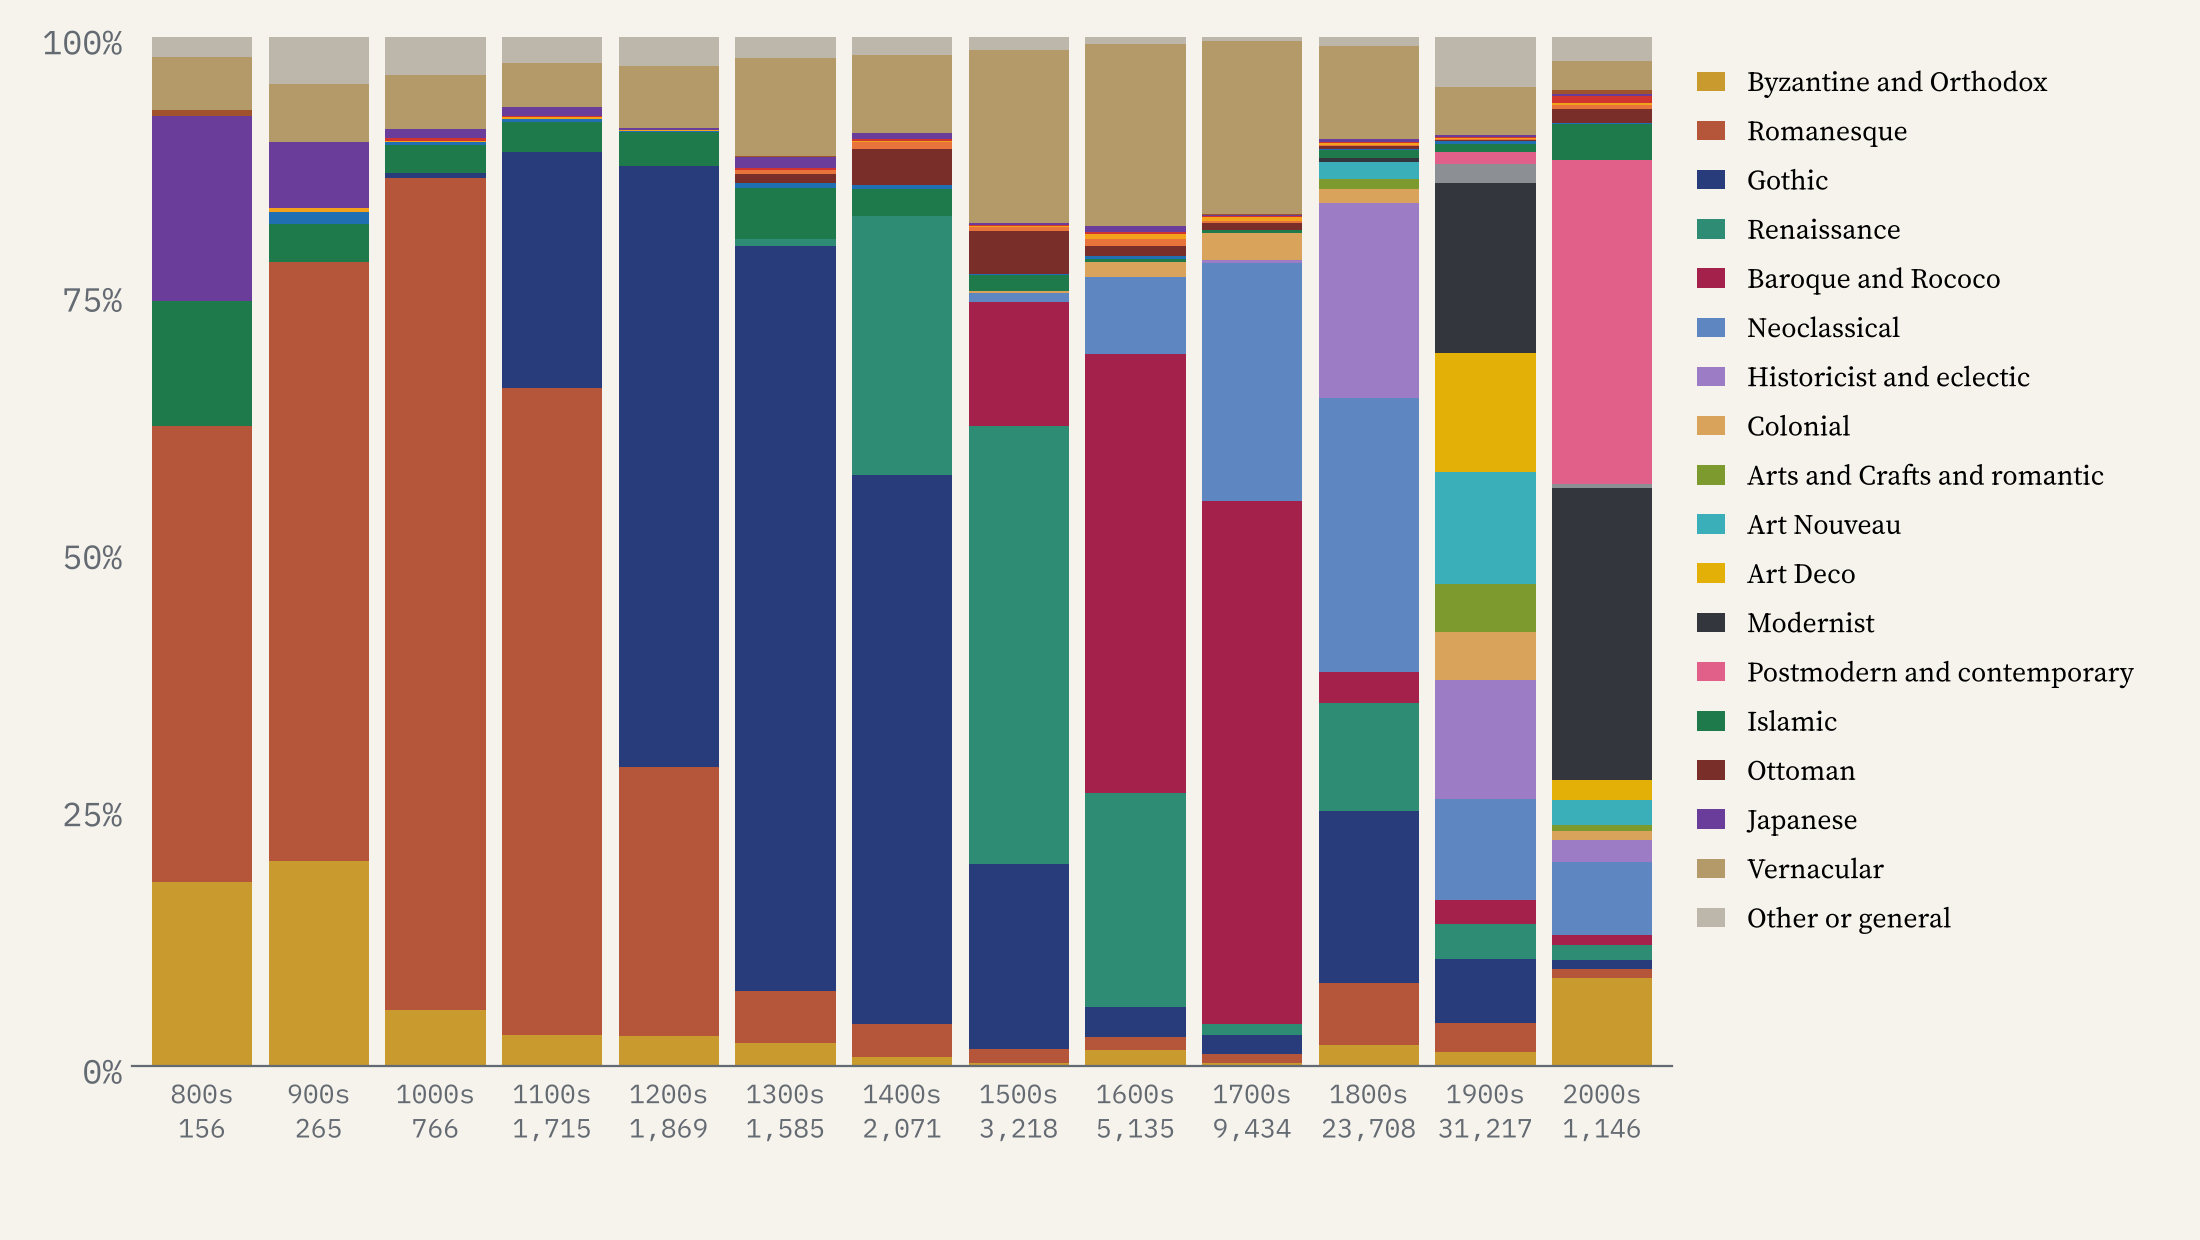
\includegraphics[width=\textwidth]{f_centuries.png}
\caption{Share of dated buildings by style family and century, with the number of buildings under each column.}\label{fig:cent}\end{figure}

\begin{figure}[tbp]\centering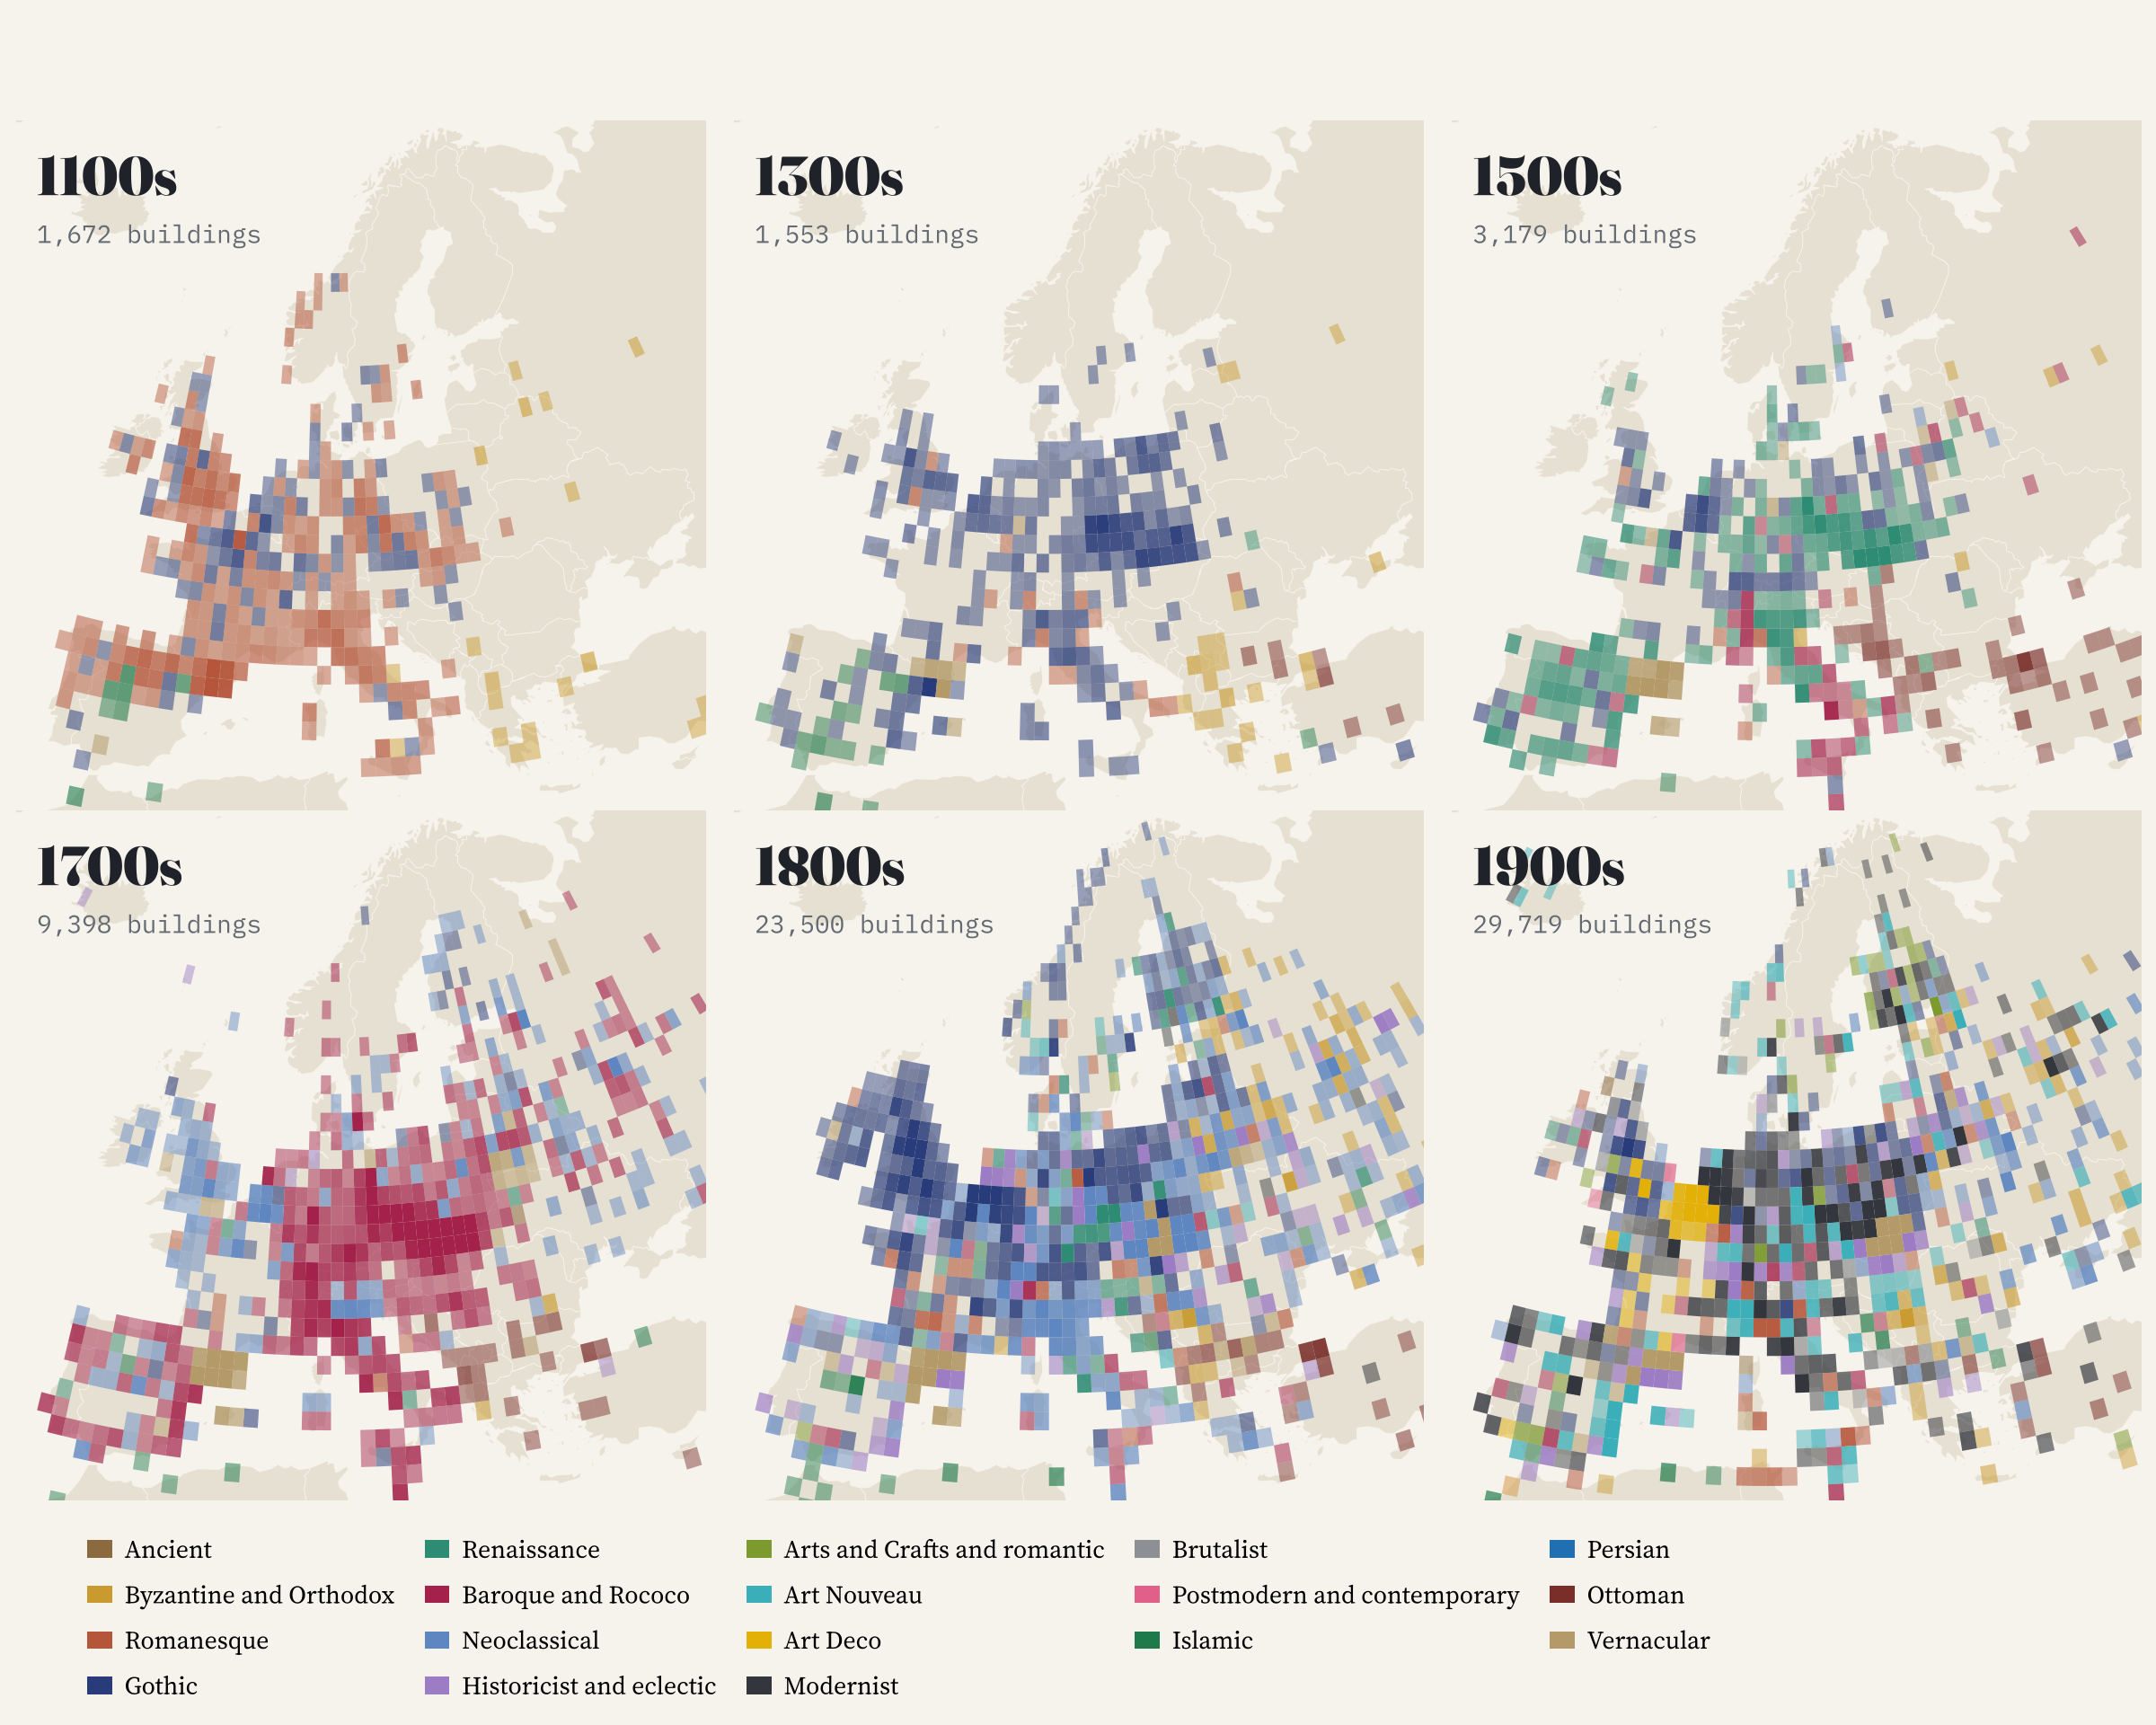
\includegraphics[width=\textwidth]{f_europe_centuries.png}
\caption{Dominant style family in each 1-degree square of Europe, for buildings begun in six centuries. Paler squares hold fewer buildings.}\label{fig:eur}\end{figure}

\subsection{How revivals travelled}
Gothic Revival is the largest revival: 10,776 buildings in 97 countries, 40\% outside Europe. The United States has the most (3,426), ahead of Germany (1,384), Poland (1,219) and the United Kingdom (1,175). The dates follow the revival outward from Britain (Table~\ref{tab:gr}, Figure~\ref{fig:gr}): the first tenth of British buildings were begun by 1832, of Canadian by 1848, Australian by 1849, American by 1854 and New Zealand's by 1864. The United States kept building it longest (median 1896, against 1870 in Britain). Russia's early tenth reflects the `pseudo-Gothic' palaces and churches of the 1770s and 1780s, such as Chesme and Tsaritsyno.

Other revivals were more concentrated. Of 5,518 Greek Revival buildings, 96\% are in the United States. Colonial, Spanish Colonial, Mission and related revivals (5,196 buildings) are 81\% American, with Brazil second. Moorish Revival is the most dispersed relative to its size: 407 buildings in 46 countries, led by Spain and the United States.

\begin{table}[tbp]\centering\small\caption{Gothic Revival buildings dated to a year from 1740 on, by country (at least 15): year by which the first tenth were begun, and median year.}\label{tab:gr}\begin{tabular}{llrrr}\toprule Country & Continent & Buildings & First tenth & Median\\\midrule
Russia & Europe & 84 & 1784 & 1894\\
Latvia & Europe & 35 & 1801 & 1863\\
Belarus & Europe & 33 & 1801 & 1893\\
Finland & Europe & 72 & 1806 & 1878\\
Ireland & Europe & 64 & 1823 & 1855\\
Ukraine & Europe & 16 & 1824 & 1890\\
United Kingdom & Europe & 892 & 1832 & 1870\\
Switzerland & Europe & 49 & 1844 & 1882\\
Canada & North America & 396 & 1848 & 1880\\
Australia & Oceania & 45 & 1849 & 1871\\
Czech Republic & Europe & 165 & 1850 & 1880\\
Slovakia & Europe & 48 & 1851 & 1889\\
Austria & Europe & 19 & 1853 & 1875\\
Belgium & Europe & 225 & 1853 & 1892\\
Brazil & South America & 25 & 1853 & 1898\\
France & Europe & 240 & 1854 & 1877\\
Germany & Europe & 416 & 1854 & 1886\\
United States & North America & 1,454 & 1854 & 1896\\
Poland & Europe & 336 & 1857 & 1894\\
Norway & Europe & 48 & 1858 & 1881\\
Italy & Europe & 146 & 1860 & 1898\\
Netherlands & Europe & 114 & 1861 & 1887\\
New Zealand & Oceania & 45 & 1864 & 1884\\
Spain & Europe & 52 & 1870 & 1897\\
\bottomrule\end{tabular}\end{table}

\begin{figure}[tbp]\centering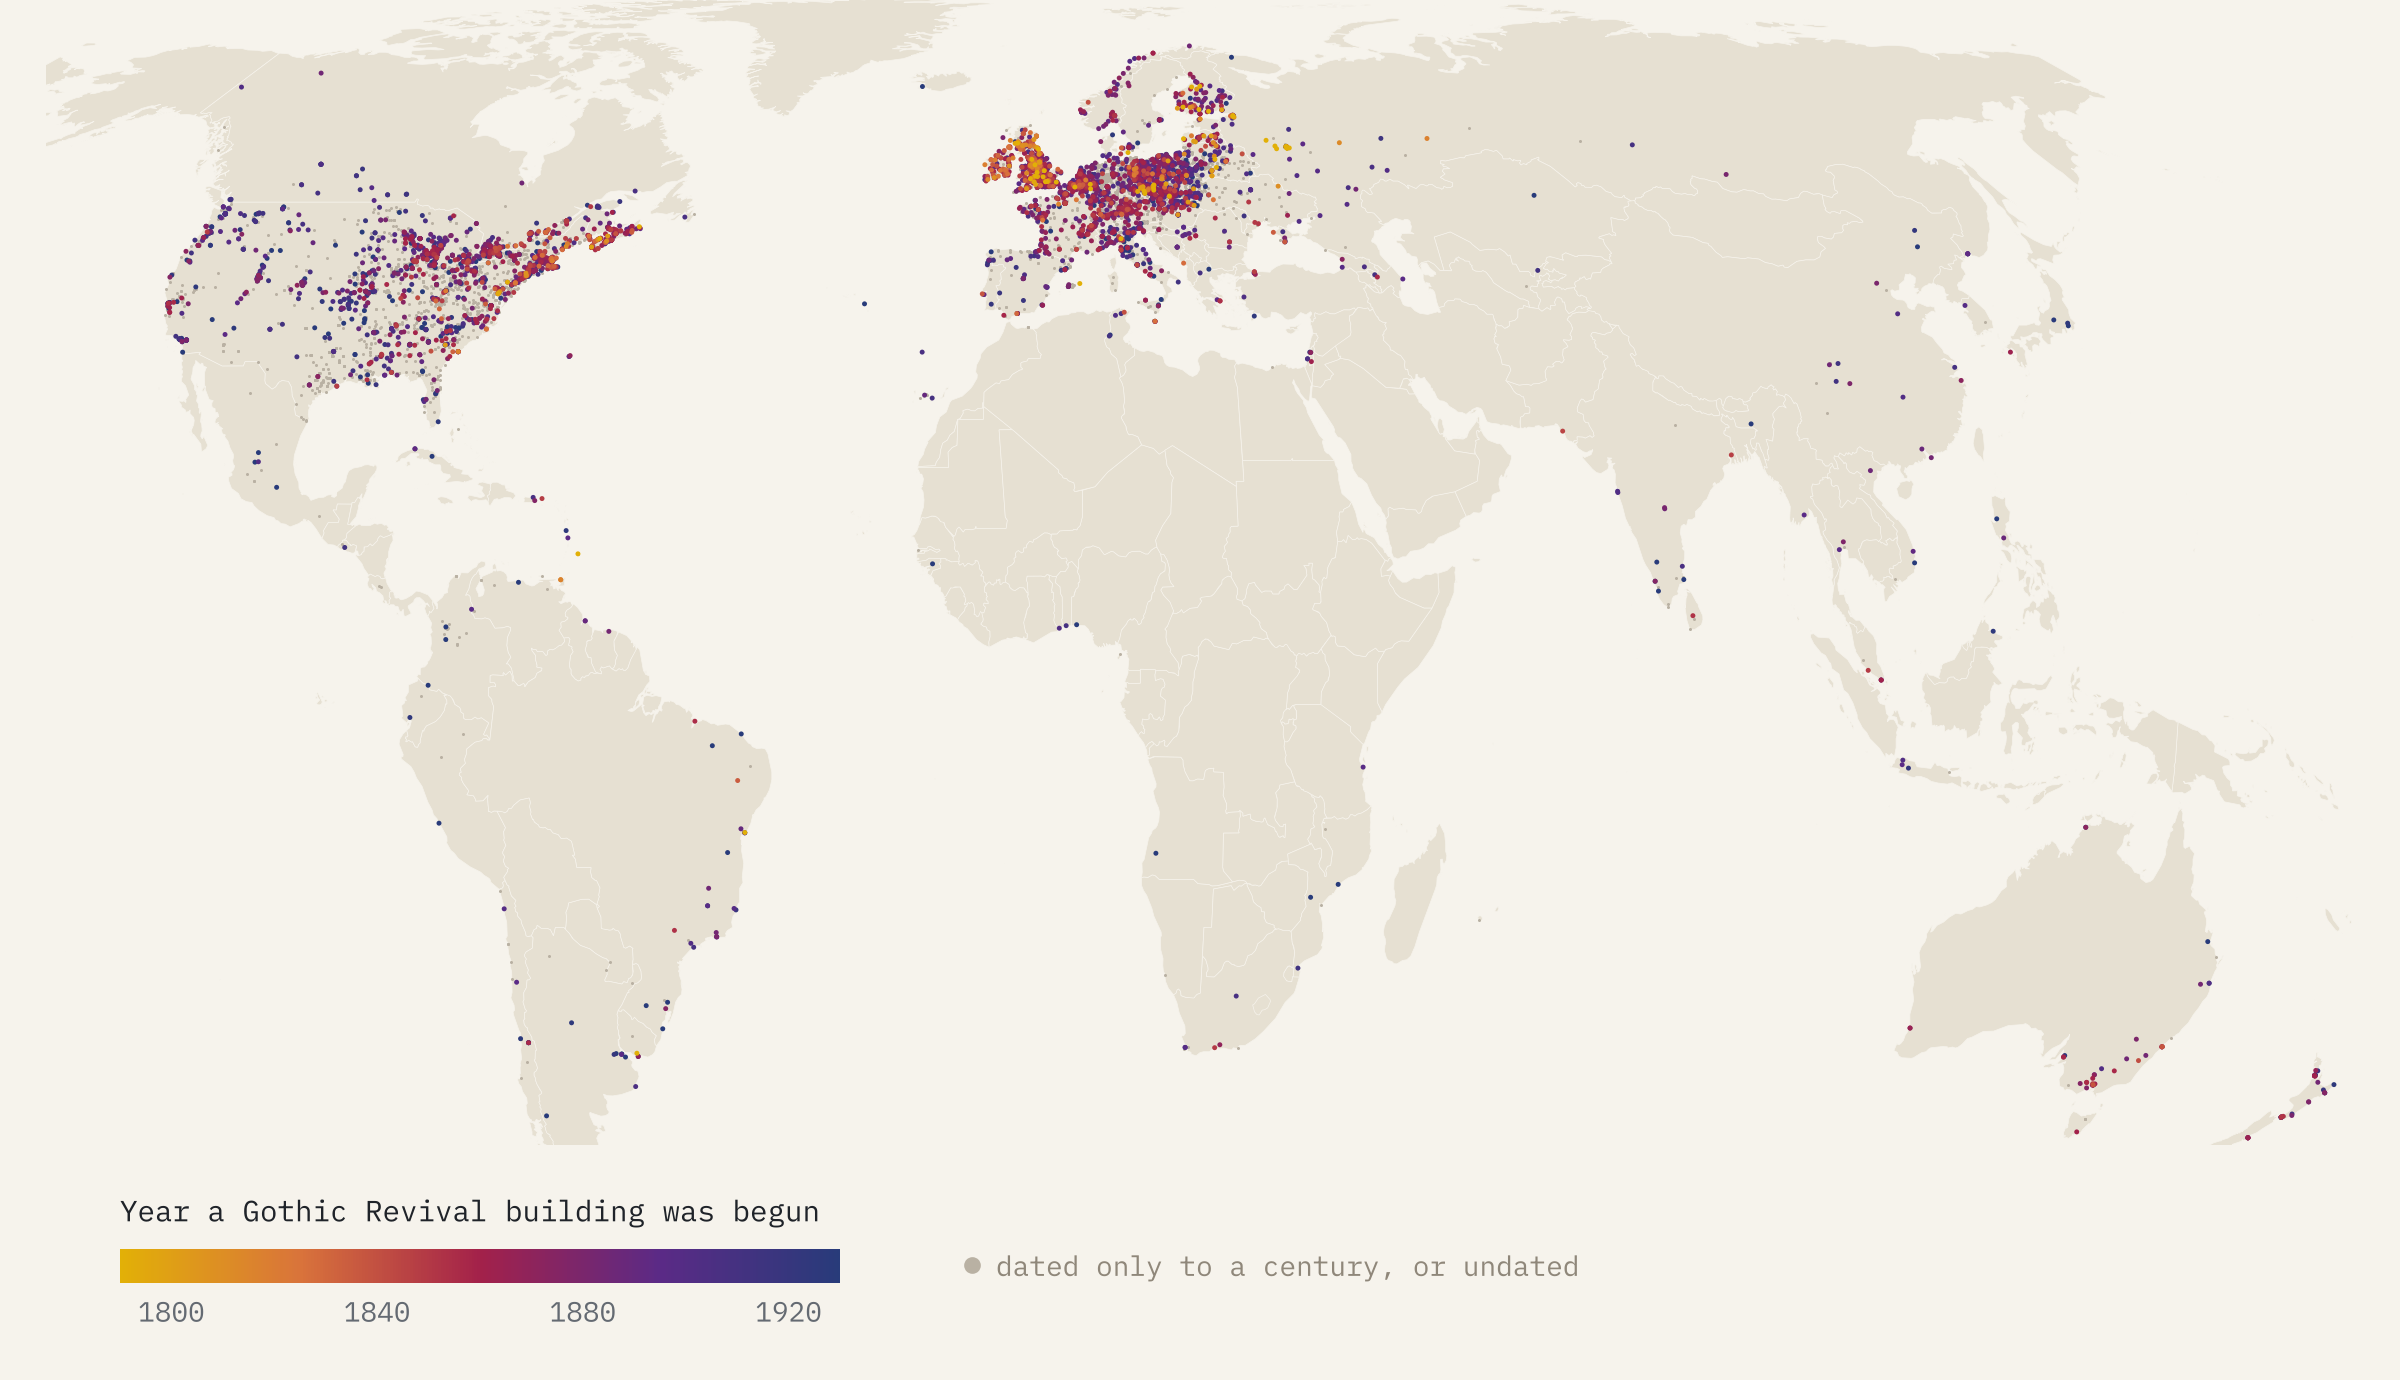
\includegraphics[width=\textwidth]{f_gothic_revival.png}
\caption{Gothic Revival buildings coloured by the year they were begun (years only; buildings dated only to a century, or undated, in grey).}\label{fig:gr}\end{figure}

\subsection{Capitals}
Of 53 national capitals with at least 40 buildings within 15 km, Neoclassical is the most common family in 6: Helsinki, Washington, Tbilisi, Paris, London and Havana. Helsinki has the highest Neoclassical share (32.5\%), reflecting the Empire-style centre built after it became capital of the Grand Duchy of Finland, followed by Dublin, Minsk, Santiago and Washington (Figure~\ref{fig:cap}).

\begin{figure}[tbp]\centering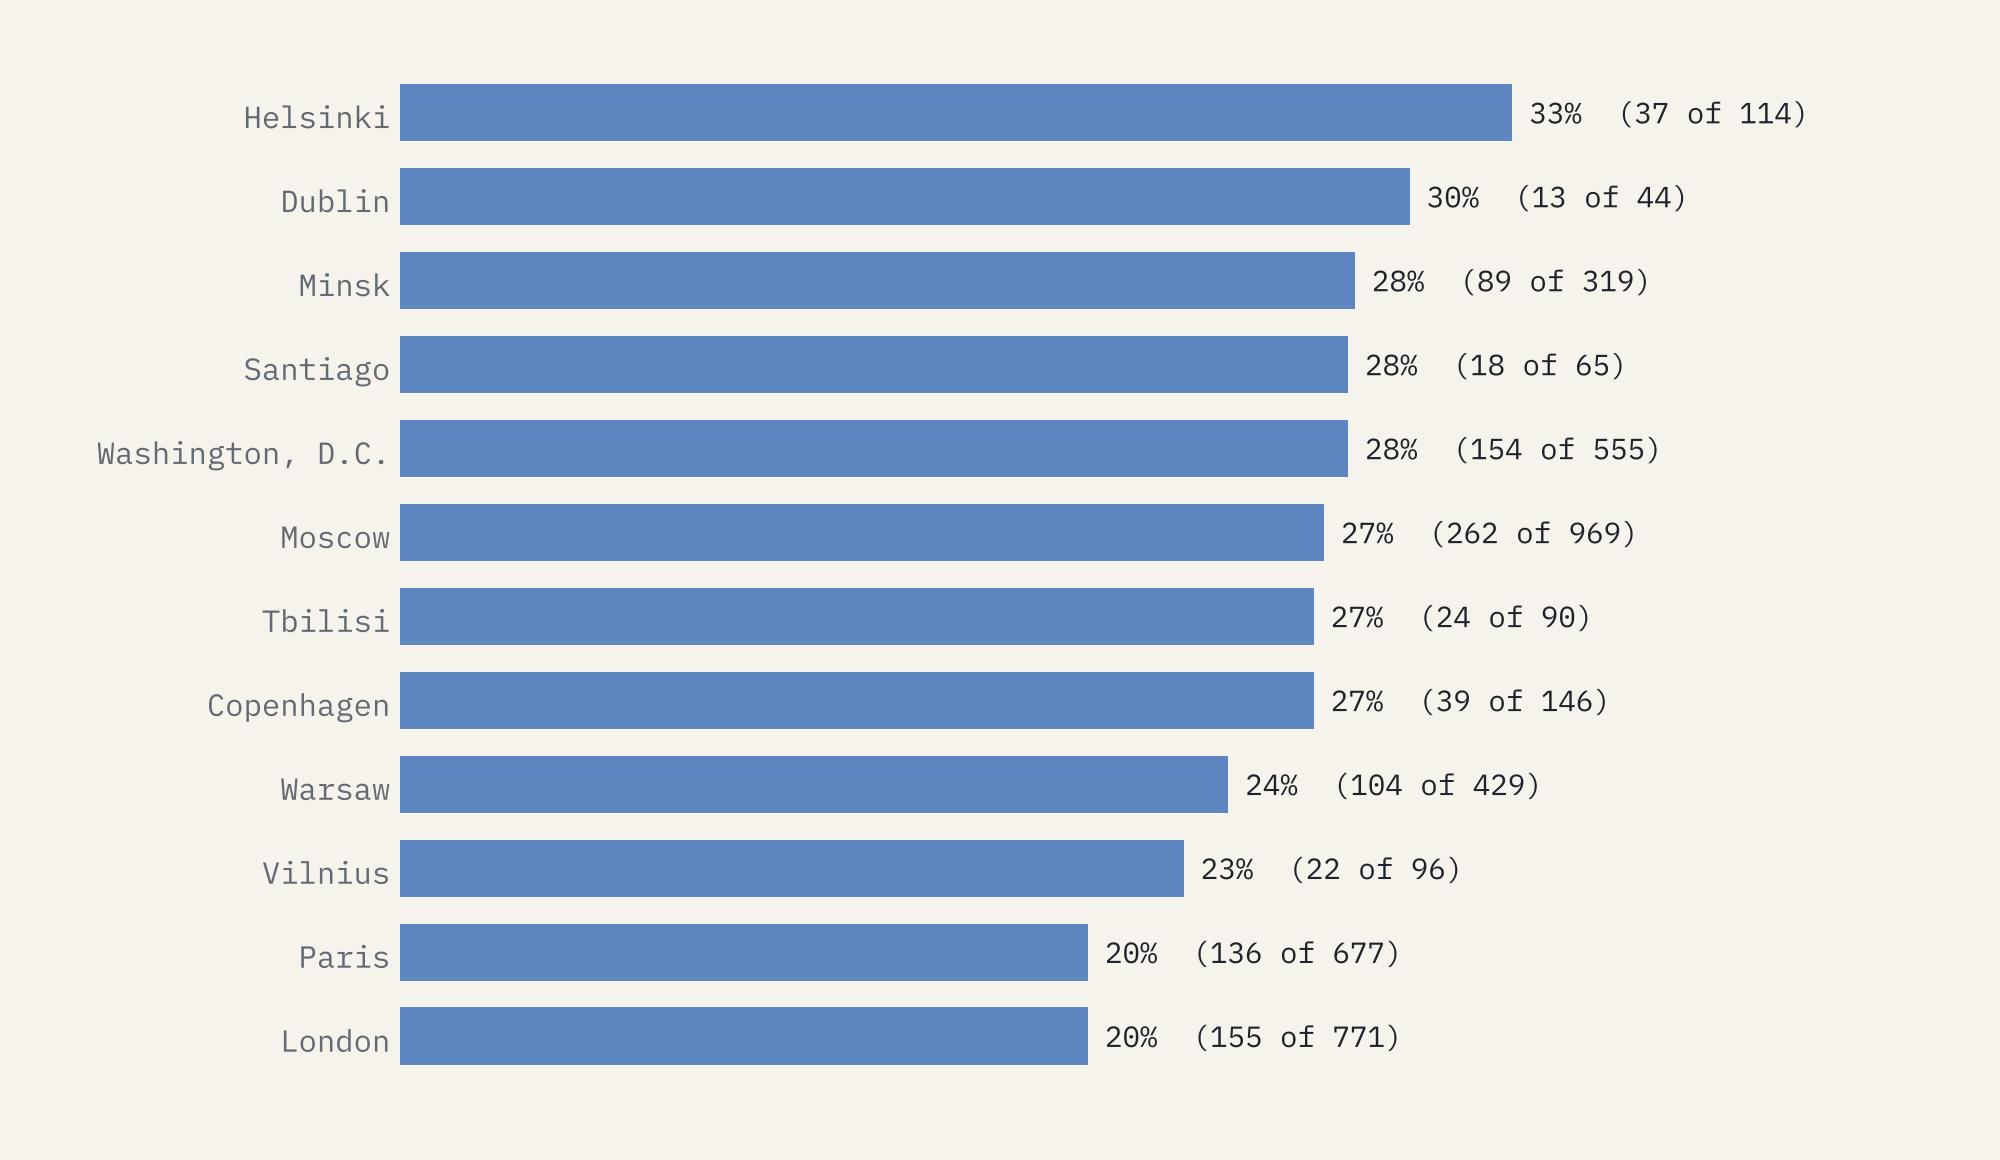
\includegraphics[width=.84\textwidth]{f_capitals.png}
\caption{Neoclassical share of buildings within 15 km of national capitals (top 12 of 53).}\label{fig:cap}\end{figure}

\subsection{Coverage}
The record is concentrated (Figure~\ref{fig:cov}). The United States (22.3\%) and Spain (20.7\%) hold 43\% of all buildings; Germany, Italy and Slovakia follow, and the top five countries hold 60.8\%. Germany, France and the United Kingdom together hold 12.1\%. Spain's total includes 5,782 Catalan farmhouses (masies) and 675 grain silos; Slovakia has the most buildings per head of any country with over two million people (1,923 per million), and only 11\% of its items have an English label. By continent Europe holds 67.9\%, North America 24.0\%, Asia 5.6\%, South America 1.7\%, Oceania 0.5\% and Africa 0.4\%. China has 381 buildings with a style and India 1,116. Half of all buildings have 2 wiki pages or fewer; 17.6\% have none.

\begin{figure}[tbp]\centering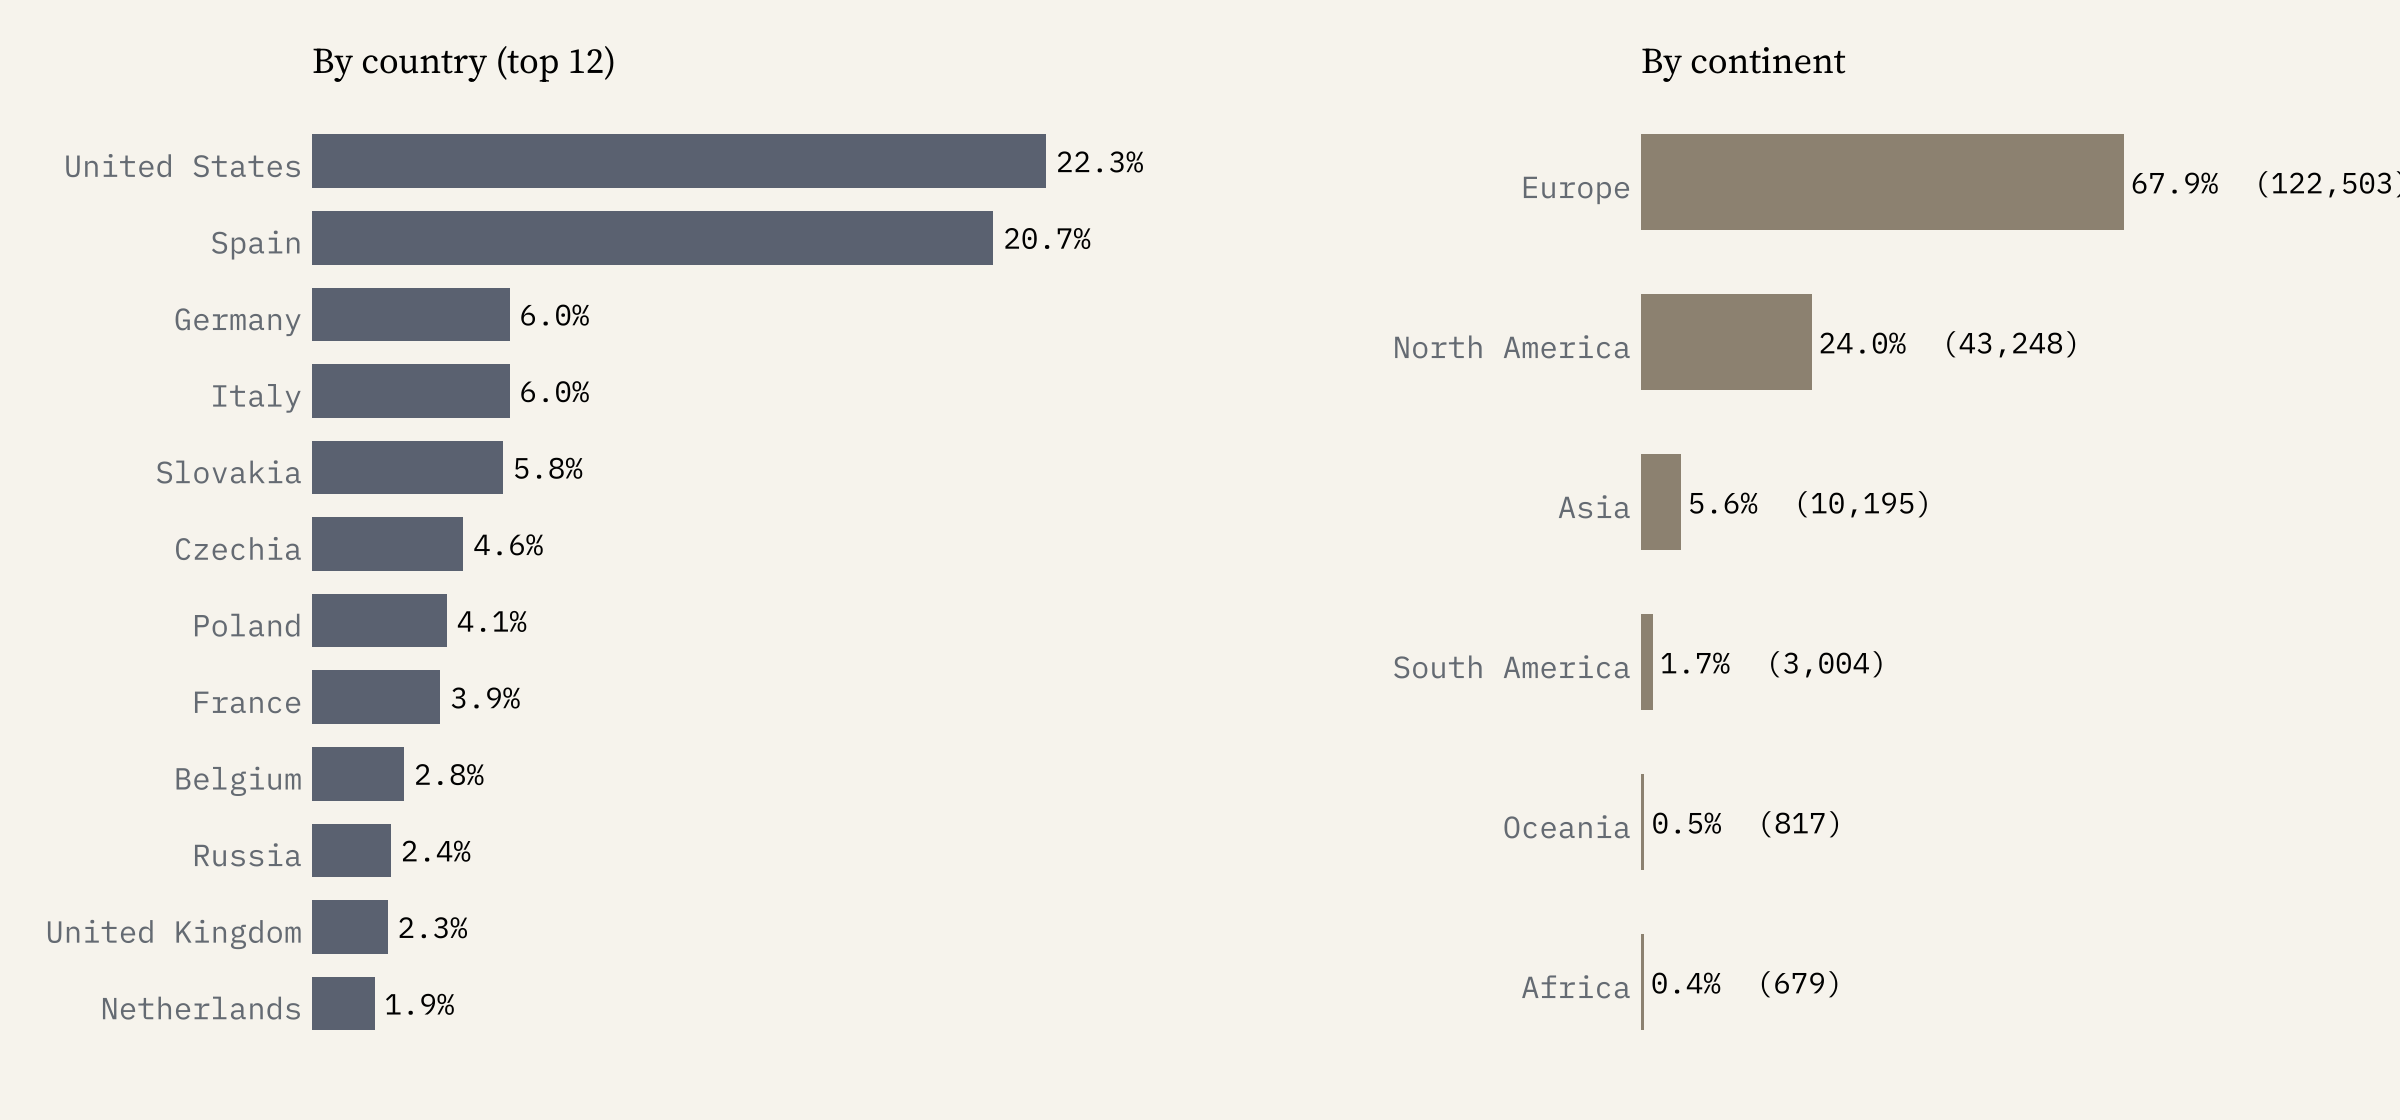
\includegraphics[width=\textwidth]{f_coverage.png}
\caption{Share of buildings by country (top 12) and continent.}\label{fig:cov}\end{figure}

\section{Discussion}
The first finding is reassuring: a crowd-sourced database, with no notion of a canon, reproduces the outline of the architectural history textbook. Romanesque, Gothic, Renaissance, Baroque, Neoclassical and Modernist each lead their centuries in turn, and the maps show Gothic consolidating in the north and Baroque in the Catholic centre of Europe. The dated buildings also show the nineteenth century as the century of revivals, and allow the spread of Gothic Revival through Britain's settler colonies and the United States to be followed decade by decade.

The second finding is about the record. The style property is used most where heritage lists appear to have been loaded in bulk, and the large blocks of American houses and courthouses, Catalan farmhouses, and Slovak, Czech and Belgian monuments leave their mark on every count, which is why Belgium's buildings are most often Art Deco and Spain's most often vernacular. Outside Europe and North America, styles are recorded mainly for famous sites, and the labels themselves are European in outlook: Iranian buildings are labelled by dynasty, Japanese shrines by roof type, and few Maya or Inca sites carry a style at all. The map is a map of attention as much as of architecture.

\section{Limitations}
First, coverage is uneven between countries and kinds of building, and nothing here is a census. Second, Wikidata's style statements are of mixed quality: overlapping labels (`Classicism', `Neoclassicism', `Neoclassical architecture'), styles of a later rebuild attached to an older building, and a few whole towns. Third, the family mapping involves judgement, especially for broad or political labels and for styles that straddle families; the full table is published so that others can change it. Fourth, dates are founding dates of uncertain precision; the reading of round-century years and the exclusion of anachronistic dates are reasonable but not exact. Fifth, sitelinks measure documentation, not importance.

\section{Conclusion}
Wikidata's architectural styles give a recognisable, if Europe-heavy, map of the world's building styles through time. Grouped into families and dated with care, they recover the familiar sequence of styles and trace how revivals travelled; read critically, they also show where the record is thin. The atlas and its data are offered as a starting point for exploration and correction.

\section*{Data and code availability}
The interactive atlas is at \url{https://maps.tristanhotham.com/architecture-styles/}. Data and code are at \url{https://github.com/Tristan-Hotham/architecture-styles} and archived with this paper at \url{https://doi.org/10.5281/zenodo.23842989}. Wikidata content is CC0; the derived data and text are released under CC BY 4.0 and the code under the MIT licence.

\section*{AI statement}
I wrote the text, with drafting and editing assistance from Claude (Anthropic), which also helped prepare the analysis code. I reviewed and checked all text and results.

\begin{thebibliography}{9}
\bibitem[Bast and Buchhold(2017)]{qlever} Bast, H. and Buchhold, B. (2017) QLever: a query engine for efficient SPARQL+text search. \emph{Proceedings of the 2017 ACM Conference on Information and Knowledge Management}, 647 to 656. \url{https://qlever.cs.uni-freiburg.de/}
\bibitem[Natural Earth(2026)]{naturalearth} Natural Earth (2026) Admin 0 countries (1:50m) and populated places (1:10m). Public domain. \url{https://www.naturalearthdata.com/}
\bibitem[Vrandečić and Krötzsch(2014)]{wikidata} Vrandečić, D. and Krötzsch, M. (2014) Wikidata: a free collaborative knowledgebase. \emph{Communications of the ACM}, 57(10), 78 to 85.
\bibitem[Wikidata(2026)]{p149} Wikidata contributors (2026) Property P149, architectural style. \url{https://www.wikidata.org/wiki/Property:P149}
\end{thebibliography}
\end{document}
